\documentclass{report}
\usepackage[utf8]{inputenc}
\usepackage{amssymb}
\usepackage{amsmath}
\usepackage[margin=1in]{geometry}
\usepackage{graphicx}

\title{Bsc notes}
\author{André O. Andersen}

\begin{document}

\maketitle

\section*{Newell et al. - Stacked Hourglass Networks for Human Pose Estimation}
\begin{itemize}
    \item We introduce a novel "stacked hourglass" network design for predicting human pose. We refer to the design as an hourglass bsed on our visualization of the steps of pooling and subsequent upsamling used to get the final output of the network. The hourglass network pools down to a very low resolution, then upsamples and combines features across multiple resolutions.
    \item We expand on a single hourglass by consecutively placing multiple hourglass modules together end-to-end. This allows for repeated bottom-up, top-down inference across scales. In conjunction with the use of intermediate supervision, repeated bidirectional inference is critical to the network's final performance. 
    \item Our hourglass module before stacking is closely connected to fully convolutional networks. Our hourglass module differs from these designs mainly in its more symmetric distribution of capacity between bottom-up processing (from high resoltuions to low resolutions) and top-down processing (from low resolutions to high resolutions)
    \item The hourglass is set up as follows: Convolutional and max pooling layers are used to process features down to a very low resolution. At each max pooling step, the network branches off and appies more convolutions at the original pre-pooled resolution. After reaching the lowest resolution, the network begins the top-down sequence of upsamping and combination of features across scales. To bring together information across two adjacent resolutions, we do nearest neighbor upsampling of the lower resolution followed by an elementwise addition of the two sets of features. The topology of the hourglass is symmetric, so for every layer present on the way down there is a corresponding layer going up. After reaching the output resolution of the network, two consecutive rounds of $1x1$ convolutions are applied to produce the final network predictions. The output of the network is a set of heatmaps where for a given heatmap the network predicts the probability of a joint's presence at each and every pixel.
    \item Operating at the full input resolution of $256x256$ requires a significant amount of GPU memory, so the highest resolution of the hourglass (and thus the final output resolution) is $64x64$, This does not affect the network's ability to produce precise joint predictions. The full network starts with a $7x7$ convolutional layer with stride 2, followed by a residual module and a round of max pooling to bring the resolution down from $256$ to $64$. 
    \item We take our network architecture further by stacking multiple hourglasses end-to-end, feeding the output of one as input into the next. This provides the network with a mechanism for repeated bottom-up, top-down inference allowing for reevaluation of initial estimates and features across the whole image.
    \item There are often multiple people visible in a given input image, but without a graphical modle or other postprocessing step the image must convey all necessary information for the network to determine which person deserves the annotation. We deal with this by training the network to exclusively annotate the person in the direct center.
\end{itemize}

\section*{poti et al. - Everything you wanted to know about Deep Learning for Computer Vision but were afraid to ask}
\subsection*{Abstract}
\begin{itemize}
    \item This paper has the objective to introduce the most fundamental concepts of Deep Learning for Computer vision in particular CNNs, AEs and GANs, including architectures, inner workings and optimization.
\end{itemize}
\subsection*{Convolutional Neural Networks}
\subsubsection*{A. Convolutional Layer}
\begin{itemize}
    \item A layer is composed of a set of filters, each to be applied to the entire input vector. Each fliter is nothing but a matrix $k \times k$ of weights (or values) $\mathbf{w}_i$. Each weight is a parameter of the model to be learned.
    \item Each filter will produce what can be seen as an affine transformation of the inpuit. Another view is that each filter produces a linear combination of all pixel values in a neighbourhood defined by the size of the filter. Each region that the filter processes is called local receptive field: an output value (pixel) is a combination of the input pixels in this local receptive field. In a convolutional layer, an output value $f(i, x, y)$ is based on a filter $i$ and local data coming from the previous layer centered at a position $(x, y)$.
    \item The most commonly used filter sizes are $5 \times 5 \times d$, $3 \times 3 \times d$ and $1 \times 1 \times d$, where $d$ is the depth of the tensor.
    \item It is important to mention that the convolutional operator can have different strides, which defines the step taken between each local filtering. The default is 1, in this case all pixeels are considered in the convolution. For example, with stride 2, every odd pixel is processed, skipping the others. It is common to use an arbitrary value os stride in order to reduce the running time. 
\end{itemize}
\subsubsection*{b. Activation Function}
\begin{itemize}
    \item ReLU is often use in CNNs after convolutional ayers or fully connected layers, but can also be employed before layers in a pre-activation setting.
    \item Activation functions are not useful after Pool layers because such layers only downsamples the input data.
\end{itemize}
\subsubsection*{C. Feature or acitvation map}
\begin{itemize}
    \item Each convolutional neuron produces a new vector that passes through the activation function and it is then called a feature map. Those maps are stacked, forming a tensor that will be offered as input to the next layer
\end{itemize}
\subsubsection*{D. Pooling}
\begin{itemize}
    \item Oftne applied after a few convolutional layers, it downsamples the image in order to reduce the spatial dimensionality of the vector.
\end{itemize}
\subsubsection*{E. Normalization}
\begin{itemize}
    \item It is common to apply normalization to both the input data and after convolutional layers.
    \item In input data preprocessing it is common to apply a $z$-score normalization, which can be seen as a whitening process.
    \item For layer normalization there are different approaches such as the channel-wise layer normalization, that normalizes the vector at each spatial location in the input map, either within the same feature map or across consecutive channels/maps, using L1-norm, L2-norm or variation. Other methods are Local Response Normalization or Batch normalization.
\end{itemize}
\subsubsection*{F. Fully Connected Layer}
\begin{itemize}
    \item After many convolutional layers, it is common to include fully connected layers that work in a way similar to a hidden layer in order to learn weights to classify the representation. It takes as input the reshaped (flatten) version of the data coming from the last layer
    \item The last layer of a CNN is often the one that outputs thE class membership probabilities of each class using logistic regression.
\end{itemize}
\subsubsection*{G. CNN architecture and its parameters}
\begin{itemize}
    \item Typical CNNs are organized using blocks of convolutional layers followed by an activation function, eventually pooling and then a series of fully connected layers which are also followed by activation functions. Normalization of data before each layer can also be applied.
\end{itemize}
\subsubsection*{H. Loss Function}
\begin{itemize}
    \item In order to avoid ambiguity of solution, it is possible to add a new term that penalizes undesired situations, which is called regularization. The most common regularization is the L2-norm.
\end{itemize}
\subsubsection*{I. Optimization Algorithms}
\begin{itemize}
    \item \textit{Stochastic Gradient Descent}: One possible solution to accelerate the process is to use approximate methods that goes through the data in samples composed of rando mexamples drawn from the original dataset, It is common to use mini-batches. By perfoming enough iteration, we assume it is possible to approximate the Gradient Descent method. In fact, SGD is a rough approximation, producing a non-smooth convergence. Because of that, variants where proposed to compensate for that, such as AdaGrad, AdaDelta and Adam. Those variants basically use the ideas of momentum and normalization, as we describe below.
    \item \textit{Momentum}: Adds a new variable $\alpha$ to control the change in the parameters $W$. It creates a momentum that prevents the new parameters $W_{t + 1}$ from deviating too much from the previous direction.
\end{itemize}
\subsubsection*{J. Tricks for Training CNNs}
\begin{itemize}
    \item \textit{Initialization}: Random initialization of weights is important the convergence of the network. The Gaussian distribution is often used to produce the random numbers, however, for models with more than 8 convolutional layers, the use of a fixed standard deviation was shown to hamper convergence. Therefore, when using rectifiers as activation functions it is recommented to use $\mu = 0$, $\sigma = \sqrt{\frac{2}{n_l}}$, where $n_l$ is the number of connections of a response of a given layer $l$; as well as initializing all bias parameters to 0
    \item \textit{Minibatch size}: It can be an advantage to choose the batch size so that it fully occupies the GPU memory and choose the largest experimentally found step size. A recent paper used a linear scaling rule for adjusting learning rates as afunction of minibatch size, also adding a warmup scheme with large step-sizes in the first few epochs to avoid optimization problems.
    \item \textit{Dropout}: During the forward pass of the network training stage, randomly deactivate neurons of a layer with some probability $p$. This method became known as a form of regularization that prevents the network to overfit.
    \item \textit{Batch normalization}; Also used as a regularizer, it normalizes the layer activations at each batch of input data by maintaining the mean activation close to 0 and the activation standard deviation close to 1, and using parameters $\gamma$ and $\beta$ to produce a lienar transofrmation of the normalized vector. BN became a standard in the recent years, often replacing the use of both regularization and dropout.
    \item \textit{Pre-processing}: the inptu data can be pre-processed in several ways:
    \begin{enumerate}
        \item Compute the average image for the whole training data and subtracting it from each image
        \item z-score normalization
        \item PCA whitening that first tries to decorrelate the data by projecting zero-centered original data into eigenbasis, and the takes the data in the eigenbasis and divides every dimension by the eigenvalue to normalize the scale
    \end{enumerate}
\end{itemize}

\section*{Bulat et al. - Human pose estimation via Convolutional Part Heatmap Regression}
\subsection*{Abstract}
\begin{itemize}
    \item This paper is on human pose estimation using CNN. Our main contribution is a CNN cascaded architecture specifically designed for learning part relationships and spatial context , and robustly inferring pose even for the case of severe part occlusions. To this end, we propose a detection-followed-by-regression CNN cascade. The first part of our cascade outputs part detection heatmaps and the second part performs regression on these heatmaps.
\end{itemize}
\subsection*{1 Introduction}
\begin{itemize}
    \item For the case of non-visible parts though, learning the complex mapping from occluded part appearances to part locations is hard and the network has to rely on contextual information to infer the occluded parts' location. In this paper, we show how to circumvent this problem by proposing a detection-followed-by-regression CNN cascasde for articulated human pose estimation
\end{itemize}
\subsection*{3 Method}
\subsubsection*{3.1 VGG-FCN part heatmap regression}
\begin{itemize}
    \item For training on MPII, all images were cropped after centering on the person and then scaled such that a standing-up human has height 300px. All images were resized to a resolution of 380x380px. To avoid overfitting, we performed image flipping, scaling (between 0.7 and 1.3) and rotation (between -40 and 40 degrees). Both rotation and scaling were applied using a set of predefined step sizes. Augmentation were applied randomly
    \item The detectors were trained for about 50 epochs using a learninig rate progressively decreasing from $1e-3$ to $2.5 e - 5$.
    \item Architecture:
\end{itemize}
\begin{center}
    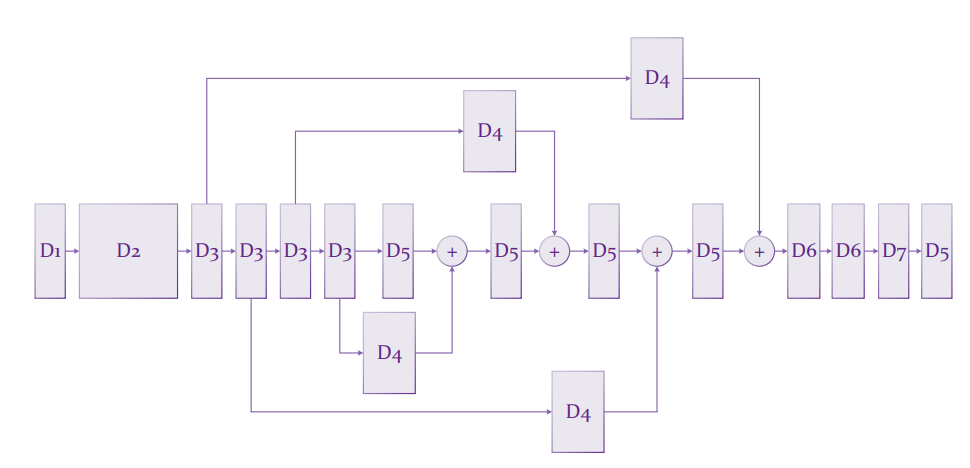
\includegraphics[height = 6 cm]{entities/bulat_1.PNG}
    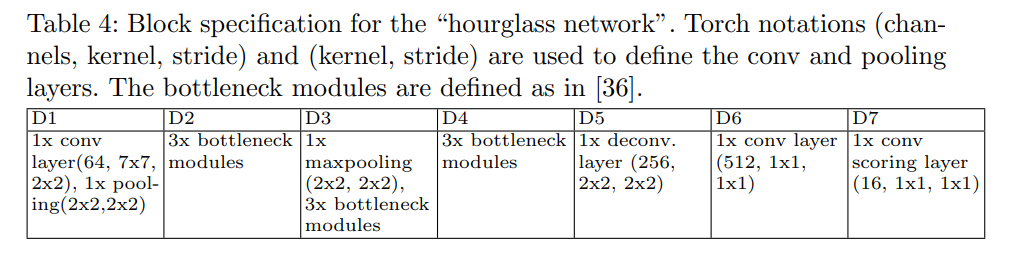
\includegraphics[height = 4 cm]{entities/bulat_2.PNG}
\end{center}
\begin{itemize}
    \item The network made us of batch normalization, and was trained with a batch size of 8.
\end{itemize}
\section*{Chu et al. - Multi-context Attention for Human Pose Estimation}
\subsection*{3. Framework}
\begin{itemize}
    \item We adopt an 8-stack hourglass network as the baseline network. it allows for repeated bottom-up, top-down inference across scales with intermediate supervision at the end of each stack. In experiments, the input iamges are $256 \times 256$, and the output heatmaps are $P \times 64 \times 64$, where $P$ is the number of body parts.
    \item We replace the residual units, which are along the side branches for combining features across multiple resolutions, by the propsed micro hourglass residual units (HRUs), and obtain a \textit{nested hourglass network}. With this architecture, we enrich the information received by the output of each building block, which makes the whole framework more robust to scale change.
    \item Wothiun each hourglass, the multi-resolution attention maps are generated from features of different scales. Attention maps are then combined to generate the refined features, which are further used to generate refined attention maps and further refined features.
    \item Different stacks are with different semantics: lower stacks focus on local apperance, while higher stacks encode global representations. Hence attention maps generated from different stacks also encode various semantic meanings. Deeper stacks with global representations are able to recover occlusions.
\end{itemize}
\section*{Yang et al. - Learning Feature Pyramids for Human Pose Estimation}
\subsection*{1. Introduction}
\begin{itemize}
    \item To enhance the robustness of DCNNs against scale variations of visual patterns, we design a \textit{Pyramid Residual Module} to explicitly learn convolutional filters for building feature pyramids. Given input features, the Pyramid Residual Module obtains features of different scales via subsampling with different ratios. Then convolution is used to learn filters for features in dfifferent scales. The filtered features are upsampled to the same resolution and are summed together for the following processing. 
\end{itemize}
\subsection*{2. Related Work}
\begin{itemize}
    \item Good initalization is essential for training deep models. Hinton and Salakhutdinov adopted the layer-by-layer pretraining strategy to train a deep autoencoder. Krizhevsky et al. initalized the weight of each layer by drawing samples from a Gaussian distribution with zero mean and 0.01 standard deviation. However, it has difficulty in training very deep networks due to the instability of gradients. Xavier initialization has provided a theoretically sound estimation of the variance of weight. It assumes that the weights are initialized close to zero, hence the nonlinear activations like Sigmoid and Tanh can be regarded as linear functions. This assumption does not hold for rectifier activations. Thus He et al. proposed an initialization scheme for recitfier networks. All the above initialization methods are derived for plain networks with only one branch.
\end{itemize}
\subsection*{4. Training and Inference}
\subsubsection*{4.1 Initializatio Multi-Branch Networks}
\begin{itemize}
    \item Initialization is essential to train very deep networks, especially for tasks of dense prediction, where Batch Normalization is less effective because of the small minibatch due to the large memory consumption of fully convolutional networks.
\end{itemize}
\section*{5. Experiments}
\subsection*{5.1 Experiments on Human Pose Estimation}
\subsubsection*{Implementation details}
\begin{itemize}
    \item The input image is $256 \times 256$ cropped from a resized image according to the annotated body position and scale. We simply use the iamge center as the body position, and estimate the body scale by the image size. Trainign data are augmneted by scaling, rotation, flipping, and adding color noise. We use a mini-batch size of 16 for 200 epochs. The learning rate is initialized as $7 \times 10^{-4}$ and is dropped by 10 at the 150th and the 170th epoch.
\end{itemize}
\section*{Tang et al. - Deeply Learned Compositional Models for Human Pose Estimation}
\subsection*{1 Introduction}
\begin{itemize}
    \item The most recent human pose estimation systems have adopted CNN as thir backbones and yielded drastic improvements on standard benchmarks. However, they are still prine to fail when there exist ambiguities caused by overlapping parts, nearby persons and clutte rbackgrounds.
\end{itemize}

\section*{Aljalbout et al. - Clustering with Deep Learning:
Taxonomy and New Methods}

\begin{itemize}
    \item The performance of current clustering methods is however highly dependent on the input data. Dif-
    ferent datasets usually require different similarity measures and separation techniques. As a result,
    dimensionality reduction and representation learning have been extensively used alongside cluster-
    ing in order to map the input data into a feature space where separation is easier. By utilizing deep
    neural networks (DNNs), it is possible to learn non-linear mappings that allow transforming data
    into more clustering-friendly representations without manual feature extraction/selection.
\end{itemize}
\begin{center}
    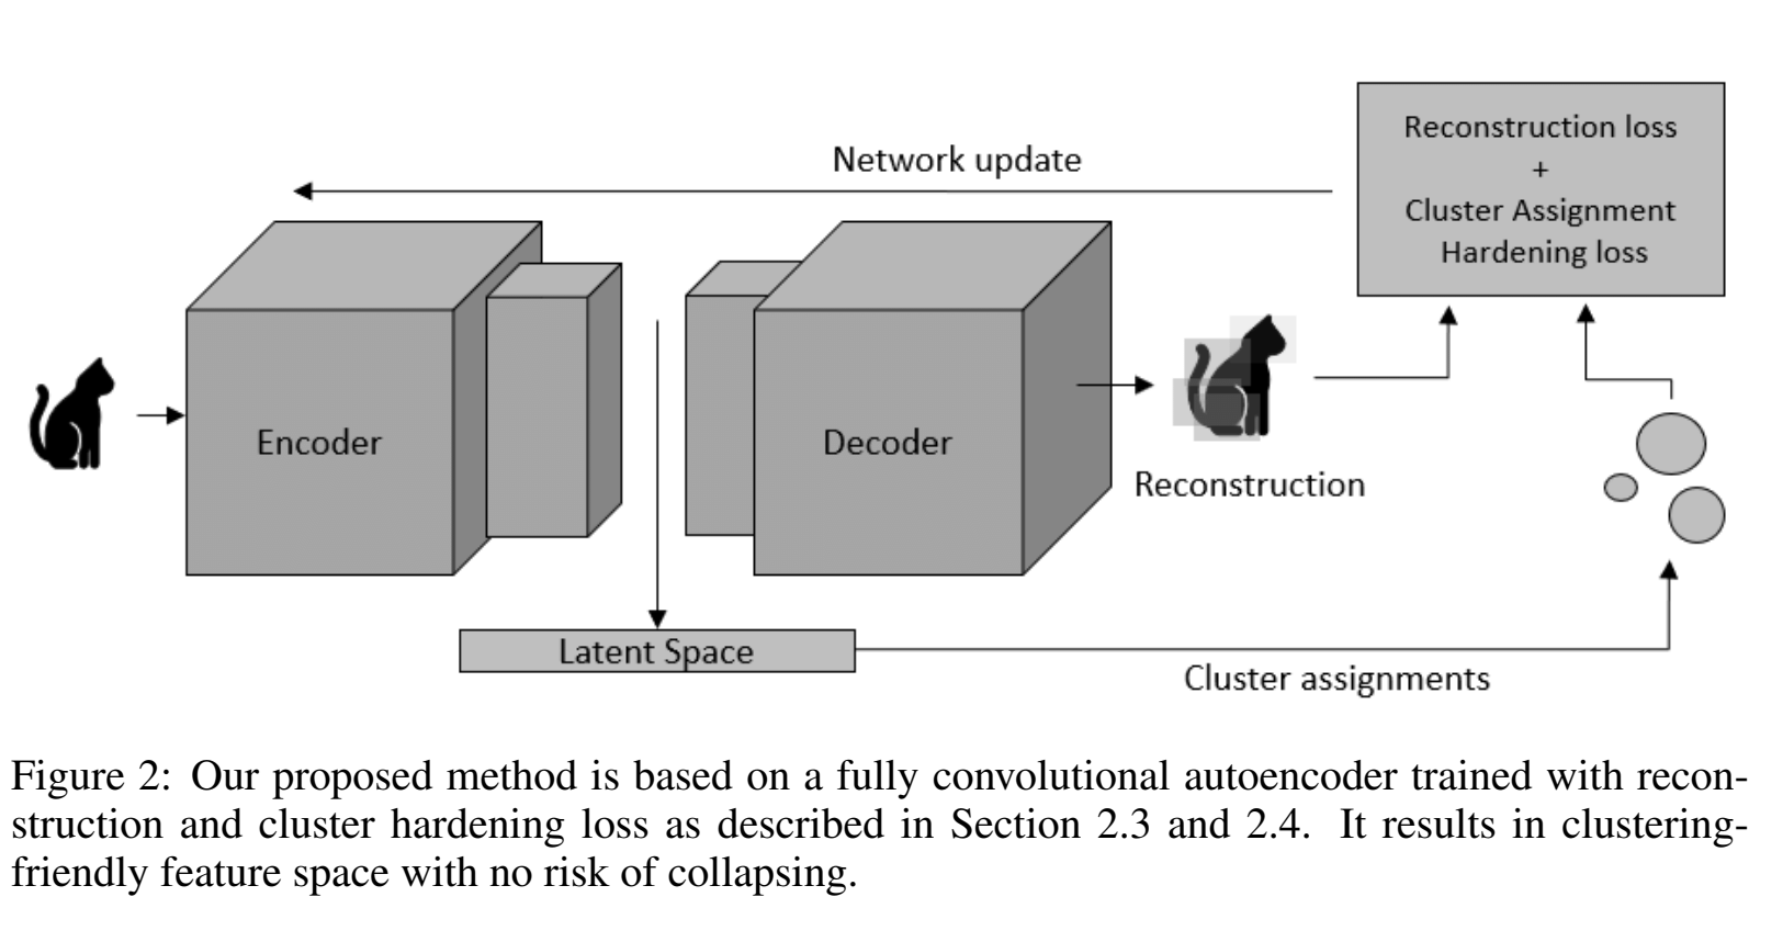
\includegraphics[height = 4 cm]{entities/Aljalbout.PNG}
\end{center}

\section*{MIN et al. - A Survey of Clustering With Deep Learning: From
the Perspective of Network Architecture}
\begin{itemize}
    \item Clustering is a fundamental problem in many data-driven application domains, and clustering
    performance highly depends on the quality of data representation. Hence, linear or non-linear feature
    transformations have been extensively used to learn a better data representation for clustering. In recent years,
    a lot of works focused on using deep neural networks to learn a clustering-friendly representation, resulting
    in a significant increase of clustering performance.
    \item Conventional clustering methods usually have poor performance on high-dimensional data, due to the inefficiency of similarity
    measures used in these methods. Furthermore, these meth-
    ods generally suffer from high computational complexity on
    large-scale datasets.
    \item The second category is based on feed-forward net-
    works trained only by specific clustering loss, thus we refer to
    this type of DNN as Clustering DNN (CDNN). The network
    architecture of this category can be very deep and networks
    pre-trained on large-scale image datasets can further boost
    its clustering performance.
    \item Although unsupervised pre-training provides a better initial-
    ization of networks, it is still challenging to extract feasible
    features from complex image data. Guérin et al. conduct extensive experiments by testing the performance of combinations of different popular CNN architectures pre-trained on ImageNet [45] and different classical clustering algorithms. The experimental results show that feature extracted from deep CNN trained on large and diverse labeled datasets, combined with classical clustering algorithms, can outperform the state-of-the-art image clustering methods.
\end{itemize}

\section*{Xie et al. - Unsupervised Deep Embedding for Clustering Analysis}
\begin{itemize}
    \item In this paper, we propose Deep Embedded Clustering (DEC), a method that simultaneously learns feature representations and cluster assignments using deep neural networks. DEC learns a mapping from the data space to a lower-dimensional feature space in which it iteratively optimizes a clustering objective
    \item We transforms the data to a lower space to avoid the "curse of dimensionality". 
\end{itemize}

\section*{Zeiler et al. - Visualizing and Understanding Convolutional Networks}

\begin{itemize}
    \item Uses deconv layers
\end{itemize}

\end{document}